% !TeX root = ../main.tex
% Add the above to each chapter to make compiling the PDF easier in somexcv editors.

\chapter{Related Work}\label{chapter:theoretical_background}

\section{Hyperparameter Optimization}

Most machine learning models have parameters that have to be defined before the learning phase. They are called hyperparameters and strongly influence the behavior of the model. One example is the number of epochs of the learning phase of a neural network. There are different techniques for the optimization of hyperparameters and they all define the machine learning model as a black box function $ f $ with the hyperparameters as input and the resulting performance as output. The overall goal is to find a configuration $ \lambda_{min} $ from $ \Lambda = \Lambda_1 \times \Lambda_2 \times ... \times \Lambda_N $ that minimizes the function $ f $ with $ N $ hyperparameters with 
\begin{equation}
	\label{eq:optimization}
	\lambda_{min} = \text{arg} \min_{\lambda \in \Lambda} f(\lambda) .
\end{equation}

In our case, the function f is a machine learning algorithm that is trained on a training set and evaluated on a testing set. With this, the minimization of e.g. the loss of the model optimizes the decisions it is making which leads to better prediction results. Note that one function evaluation of f is usually very expensive as the training of a machine learning model with many parameters and weights takes much time. The data set consists of $ \{ (x_i, y_i) | x_i \in X, y_i \in Y, 0 \le i \le m \} $ with m being the number of data samples. The $ x_i $ is the input data to the model and the goal is that 
\begin{equation}
	\forall i: M(x_i) = y_i.
\end{equation}
where M is the model. In the context of supervised learning, the whole data set is split into a training set which is used to optimize the model and a testing set to evaluate the performance on new, unseen data \cite{supervised_learning}.

All in all, the goal is get evaluation scores on the testing data set which can be achieved with Equation \ref{eq:optimization}. 
\cite{feurer2019hyperparameter,bischl2021hyperparameter,yang2020hyperparameter}

In the following, different techniques for the optimization are presented and discussed with their advantages and disadvantages.

\subsection{Grid Search}
The idea of the first approach for the optimization is to discretize the domains of each hyperparameter and evaluate each combination. This suffers from the curse of the dimensionality as it scales exponentially with the number of hyperparameters. For $ d $ parameters and $ n $ values per hyperparameter, $ n^d $ different configurations are possible which all have to be evaluated. 

One advantage of this method is that it is easy to implement and very simple. Also, the whole search space is explored evenly.

On the other hand, the curse of the dimensionality makes it very slow if the function evaluations are very expensive. This is the case for most machine learning algorithms because the training phase of the model takes much time. Another drawback is that each hyperparameter only takes $ n $ different values.


\subsection{Random Search}
The next technique \cite{random_search} is similar to the grid search because the idea is also to evaluate different hyperparameter configurations. In contrast to the previous one, random search generates for each run and for each parameter exactly one random value from an interval which has to be specified. For this approach, a budget $ b $ has to be given. This parameter determines the number of different combinations that are evaluated. A direct comparison of grid search and random search can be seen in figure \ref{fig:comparison_searches}.

\begin{figure}[hbtp!]
	\centering
	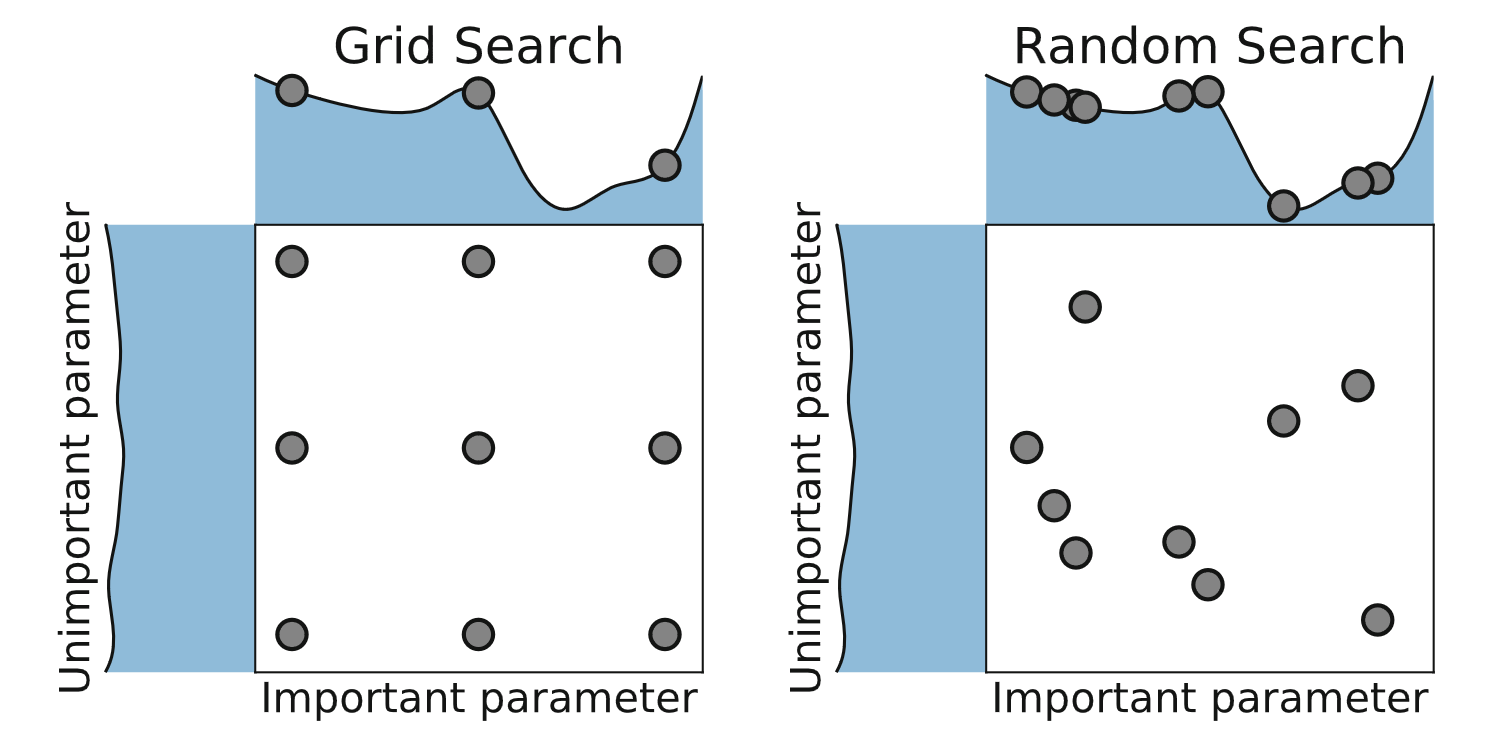
\includegraphics[scale=0.2]{figures/comparison_searches.png}
	\caption{Comparison of grid search (left) and random search (right) in the two dimensional case. For both techniques, 9 different combinations are evaluated. In the left case, only 3 distinct values for each hyperparameter are set whereas there are 9 different values for each parameter in the random search. Taken from \cite{feurer2019hyperparameter}. }
	\label{fig:comparison_searches}
\end{figure}

In this figure, a two dimensional setting is depicted. For both techniques, 9 different combinations are evaluated. In the case of grid search, only 3 distinct values are taken for each hyperparameter while there are 9 different ones in the random search. In this example, the better result is found in random search as more distinct values are taken for the important parameter. Note that this is not always the case. 

Compared to the normal grid search, this is one advantage. For each hyperparameter, $ b $ (budget) different values are taken into consideration which is much more compared to the grid search with the same overall number of combinations. Additionally, this technique is also easy to implement and relatively simple. 

One disadvantage is that it is also very expensive if the budget is high because of the long training times of machine learning models. 


\subsection{Bayesian Optimization}

Another possible technique for finding the best hyperparameters of machine learning models is called bayesian optimization (BO) \cite{snoek2012practical}. This is an iterative approach for optimizing the expensive black box function by modeling it based on observations. A so-called \textit{surrogate model} $ \hat{f} $ is made with the help of the \textit{archive} $ A $ which contains observed function evaluations. This surrogate model is created by regression and the technique which is most often used is the Gaussian process \cite{bischl2021hyperparameter} which is only suitable if the number of hyperparameters is not too high \cite{andonie2019hyperparameter}. The problem of this technique arises when some hyperparameters are categorical or integer-valued which is the reason why extra approximations can lead to worse results and special treatment is needed \cite{garrido2020dealing}. Another possible technique for the surrogate model is using random forests \cite{hutter2011sequential}. All in all, this function estimates the machine learning model depending on the hyperparameter configuration and also the prediction uncertainty $ \sigma(\lambda) $. A second function called \textit{acquisition function} $ u(\lambda)$ is built based on the prediction distribution. This $ u $ is responsible for the trade-off between exploitation and exploration. This means that configurations that lead to better model performances are exploited and values where no much information is gathered are explored. 

In each iteration, a new candidate configuration $ \lambda^+ $  is generated by optimizing the acquisition function $ u $. This $ u $ is much cheaper to evaluate than the $ f $ which includes learning of an expensive neural network which makes the optimization much easier.

The exact steps are presented in Algorithm \ref{alg:bayesian_opt} and Figure \ref{fig:bayesian_optimization} shows schematic iteration steps.

\begin{algorithm}[htbp!]
	\caption{Bayesian Optimization}\label{alg:bayesian_opt}
	\begin{algorithmic}
		\State Generate initial $\lambda^{(1)}, ..., \lambda^{(k)} $
		\State Initialize archive $A^{[0]} \gets ((\lambda^{(1)}, f(\lambda^{(1)})), ..., (\lambda^{(k)}, f(\lambda^{(k)})))$
		\State $ t \gets 1 $ 
		\While{Stopping criterion not met}
			\State Fit surrogate model $ (f(\lambda), \sigma(\lambda)) $ on $ A^{[t-1]} $
			\State Build acquisition function $ u(\lambda) $ from $ (\hat{f}(\lambda), \sigma(\lambda)) $
			\State Obtain proposal $ \lambda^{+} $ by optimizing $ u: \lambda^+ \in arg\max_{\lambda \in \Lambda} u(\lambda) $
			\State Evaluate $ f(\lambda^+)$
			\State Obtain $A^[t]$ by augmenting $ A^{[t-1]} $ with $ (\lambda^{(+)}, f(\lambda^{(+)})) $
			\State $ t \gets t+1 $
		\EndWhile
		\State return $ \lambda_{best} $: Best-performing $\lambda$ from archive or according to surrogates prediction
	\end{algorithmic}
\end{algorithm}

\begin{figure}[htbp!]
	\centering
	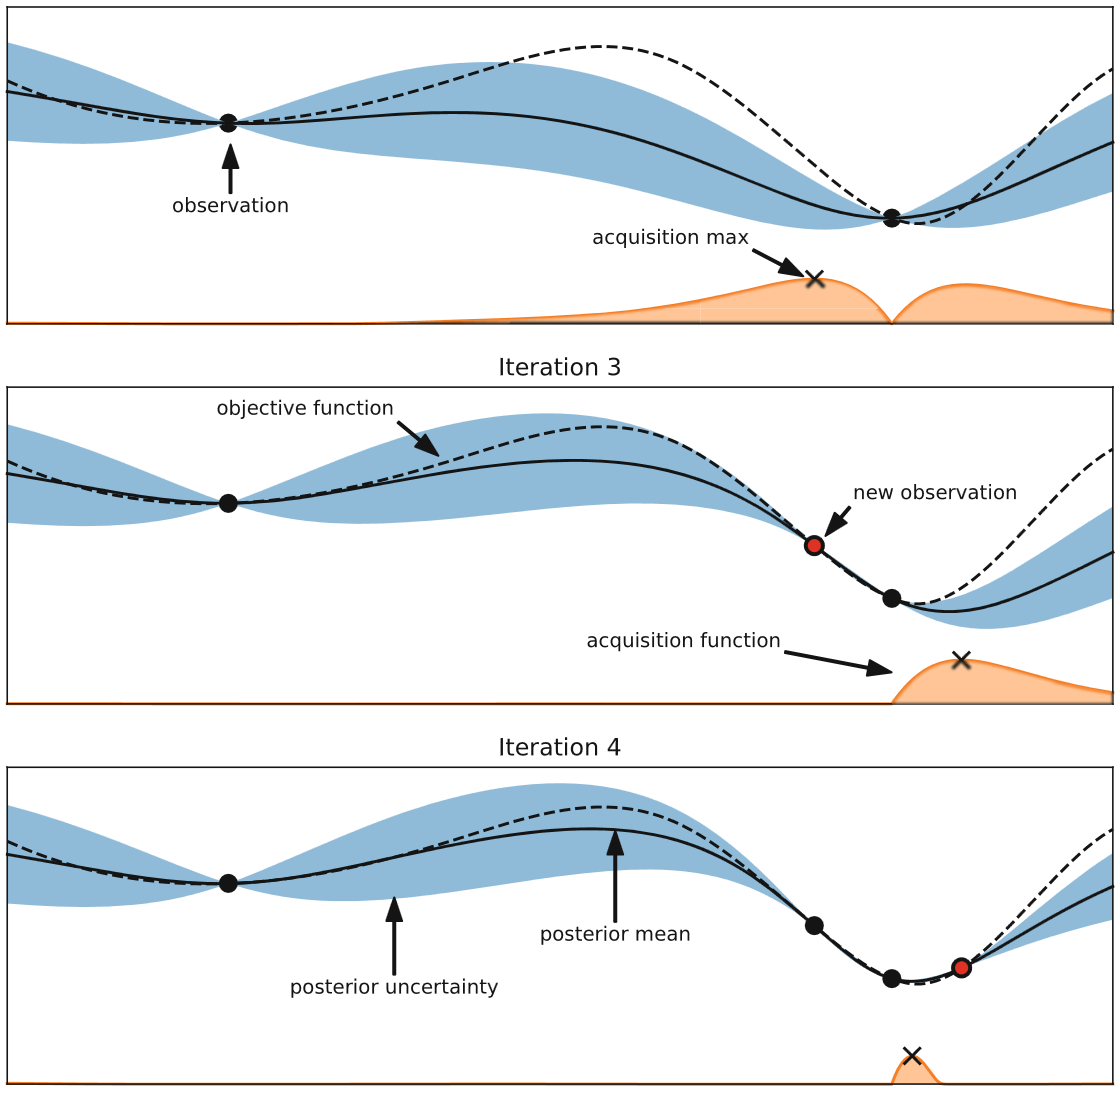
\includegraphics[scale=0.25]{figures/bayesian_optimization.png}
	\caption{ Schematic iteration steps of the bayesian optimization. The maximum of the acquisition function determines the next function evaluation (red dot in the middle). The goal is to find the minimum of the dashed line. The blue band is the uncertainty of the function. Taken from \cite{feurer2019hyperparameter}. }
	\label{fig:bayesian_optimization}
\end{figure}


First, $ k $ initial hyperparameter configurations are sampled and evaluated. This set is the starting archive $ A^{[0]} $. After that, the loop is executed as long as the stopping criterion is not met. This can be for example a budget, meaning a maximum number of function evaluations. The first step of the loop is to fit the surrogate model on the current archive. Then the acquisition function is made and optimized to get the next configuration $ \lambda^+ $. This point is evaluated and added to the archive. The overall result of the algorithm is the $ \lambda $ which is the hyperparameter configuration for the machine learning model with the overall best result.

\subsection{Other Techniques}



\section{Sparse Grids}

\subsection{Numerical Approximation of Functions}

\subsection{Adaptive Sparse Grids}
